\section{Experiment 1 : influence of the filtering of the input noise.}
For the first experiment, we use the following parameter settings : 

\begin{table}[h]
\centering
\begin{tabular}{lll}
    $ R_0 = 1000, $  &  $ f_{gen} = 0.1, $ & $ f_{noise} = \{ 0.999, 0.95, 0.6 \},$  \\
    $ \sigma_{i_0} = 0.1, $  &  $ \sigma_{n_i} = 0.1, $ & $ \sigma_{n_u} = 1.$  \\
\end{tabular}
\end{table}
The result of the first experiment are displayed on the figure~\ref{Sess1_part1_exp1}.

\paragraph{LS estimate} As can be seen on the top picture of fig.~\ref{Sess1_part1_exp1}, the LS estimate is strongly biased. This can be explained by using Eq. \ref{as_val_LS}: the  relative bias is in the order of $\frac{\sigma_{n_i}^2}{\sigma_{i_0}^2}$. With the above parameter settings, we obtain the following asymptotic value :
$$ \lim\limits_{N \rightarrow +\infty} \hat{R}_{LS} = R_0 \frac{1}{2}  = 500 $$ 
The values of the LS estimate are indeed always around 500. This bias is due to the fact that, with the LS estimate, we assume that the measured input is exact, which is not the case here because of the noise $n_i$. 

\paragraph{IV estimate} Considering Eq.~\ref{as_val_IV}, we conclude that the smaller is the ratio $\frac{R_{n_i n_i}(s)}{R_{i_0 i_0}(s)}$, the less biased is the IV estimate. 
Here, the input noise $n_i$ is generated by filtering a white noise $e_2$ by a second order Butterworth filter of parameter $f_{noise}$. 

We analyse the asymptotic value of $\hat{R}_{IV}$ in function of the parameter $f_{noise}$. Since $R_{i_0 i_0}(s)$ is kept constant, we will only talk about $R_{n_i n_i}(s)$.
\begin{itemize}
    \item if $f_{noise} = 0.999$, the generated input noise $n_i$ is a white noise. The auto-correlation function $R_{n_i,n_i}(s)$ exhibits a peak in $s = 0$ and is then absolutely 0 for all other $s$. Therefore, $R_{n_i,n_i}(1) = 0$ and the IV estimate for $s = 1$ converges to $R_0$. There is thus no bias present. On fig.~\ref{Sess1_part1_exp1} (a), we see that the mean value of IV(1) is close to $R_0$.
    \item if $f_{noise} = 0.9$, the IV estimate will have a small bias : indeed, we notice on fig.~\ref{Sess1_part1_exp1} (b.2) that the auto-correlation function $R_{n_i,n_i}(s)$ is not perfectly equal (but close) to 0 at $s=1$. The mean value IV(2) on fig.~\ref{Sess1_part1_exp1} (a) is 938 and is thus close to the searched value.
    \item if $f_{noise} = 0.6$, the bias will be bigger; $R_{n_i,n_i}(1)$ is indeed larger than in the two other cases. The mean value IV(3) on fig.~\ref{Sess1_part1_exp1} (a) is 645 and is thus far from $R_0$.
\end{itemize}

As a conclusion, the results are strongly influenced by the filter : the larger $R_{n_i,n_i}(s)$, the larger the bias will be.
\begin{figure}[h!]
    \centering
    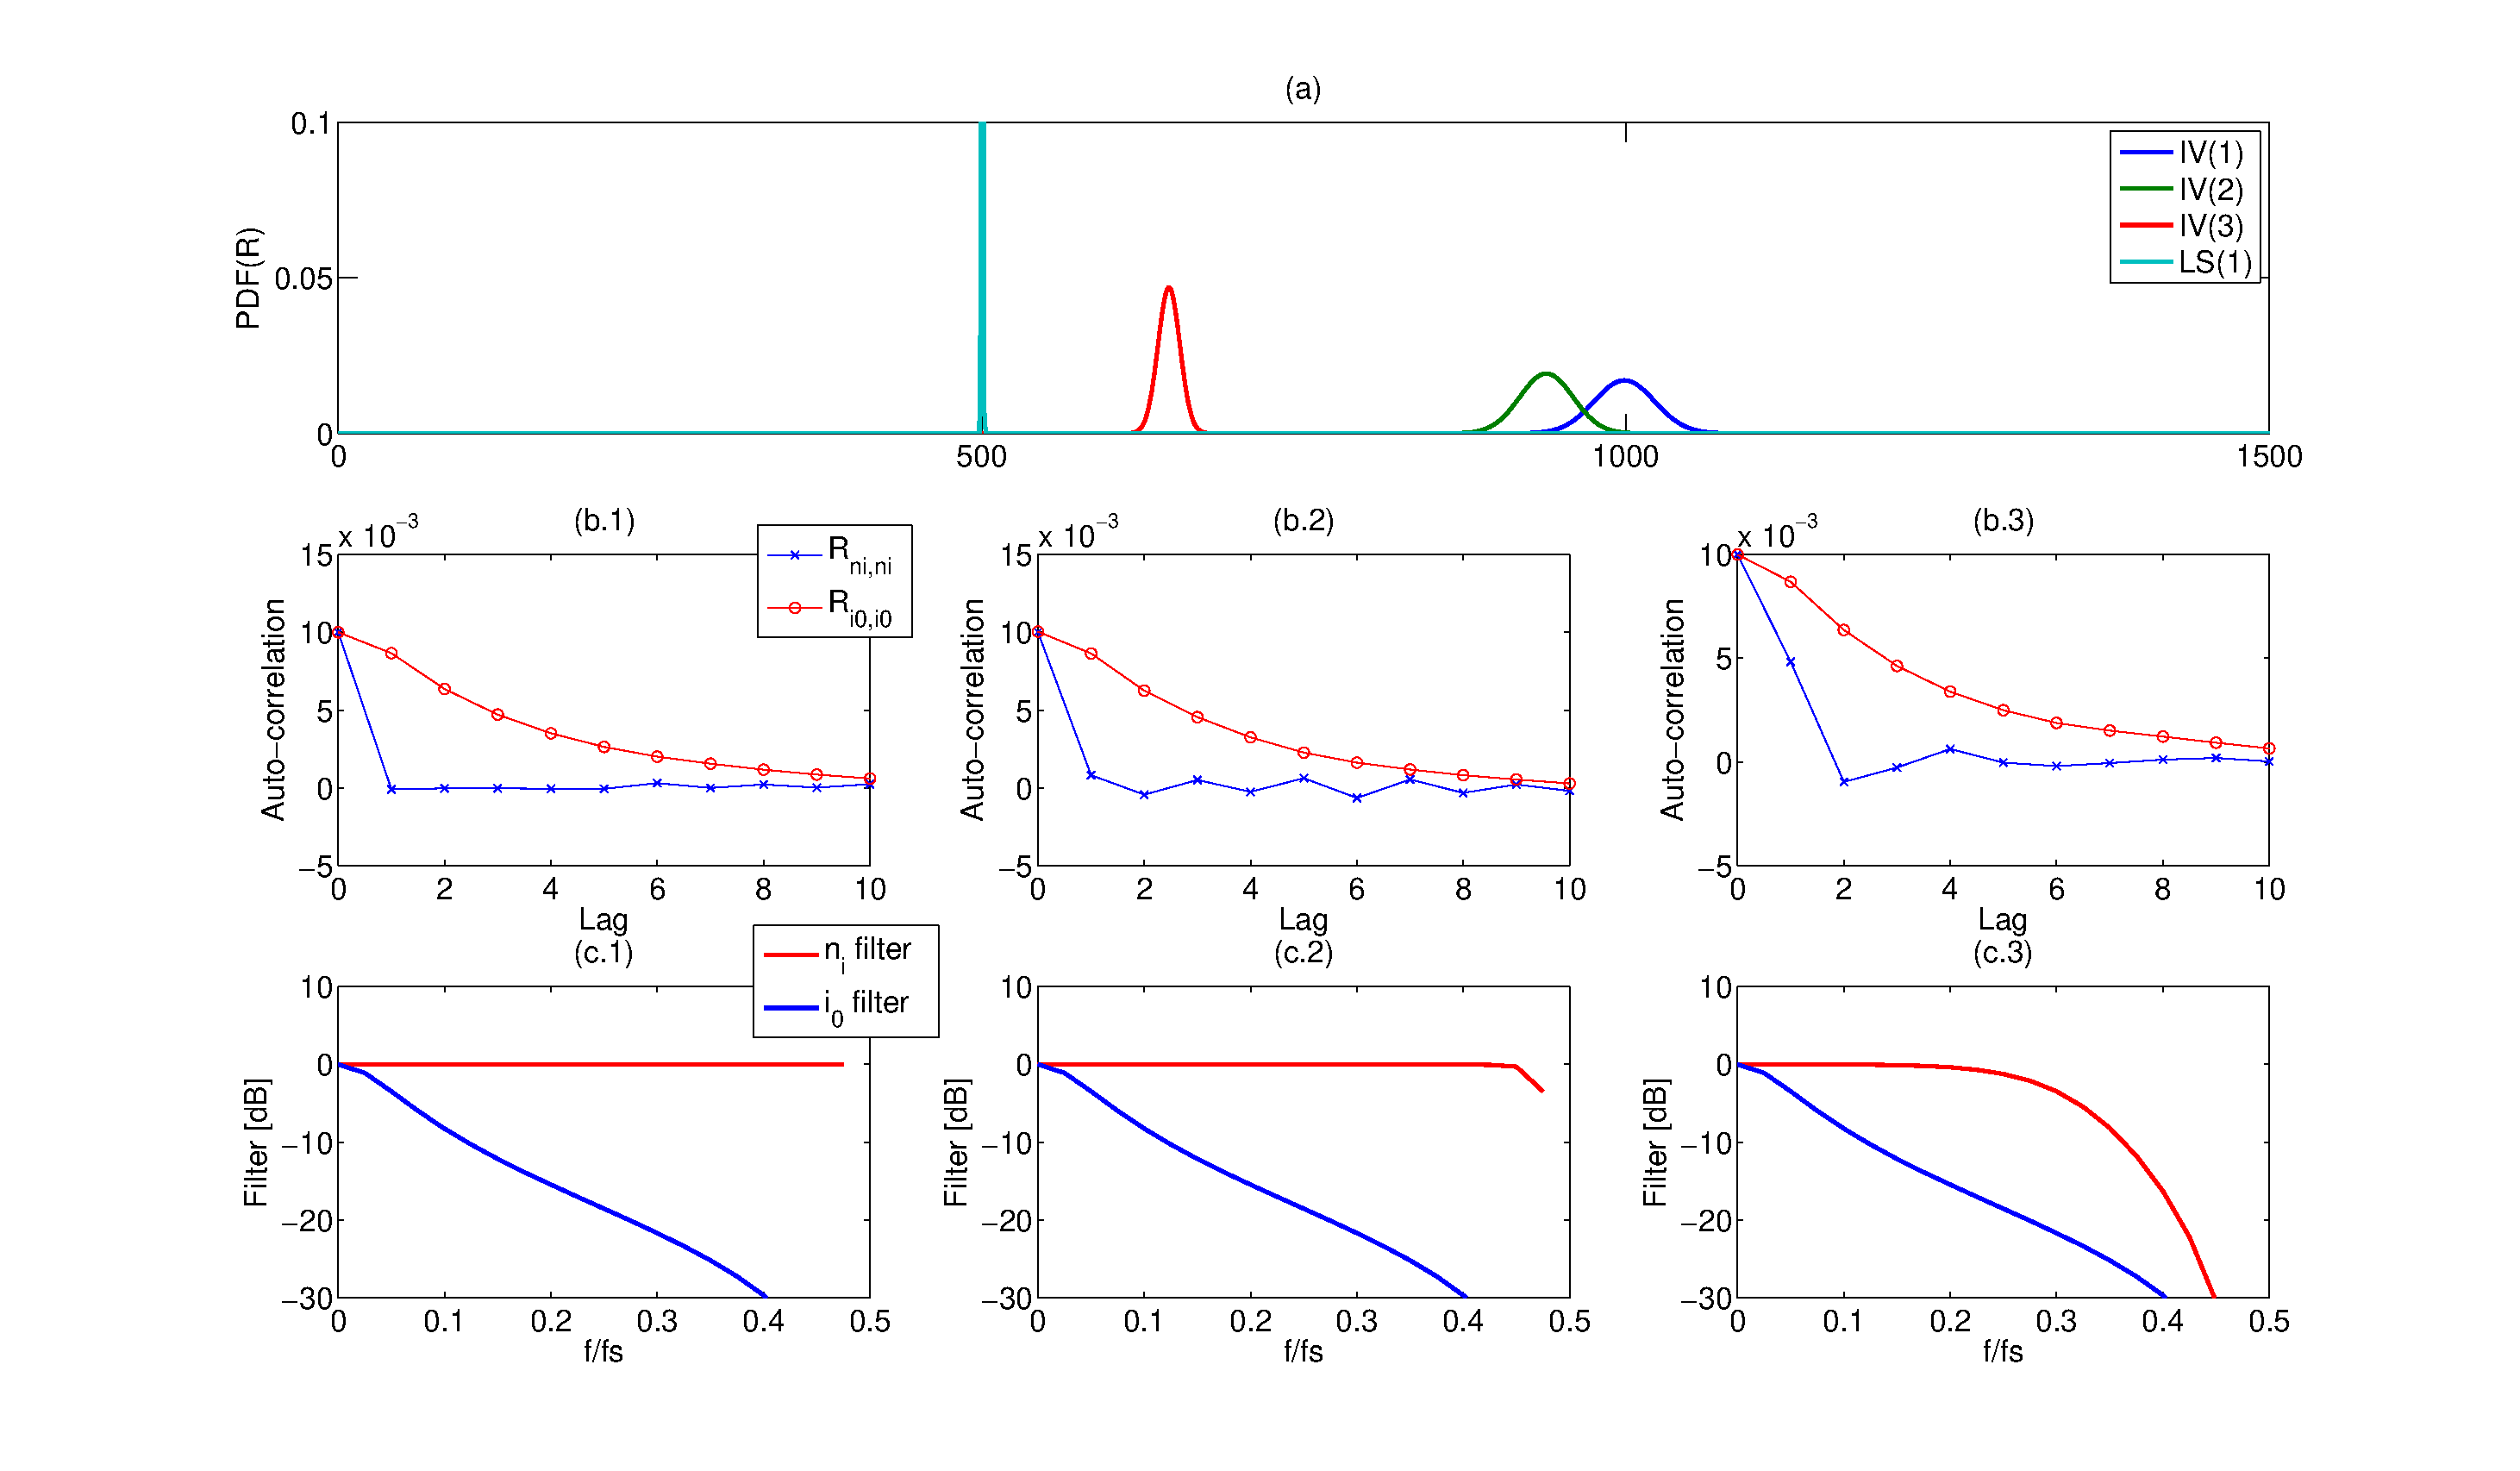
\includegraphics[width=1\textwidth]{figures/Sess1_part1_exp1.eps}
    \caption{Study of the LS and IV estimates for a varying noise filter bandwidth and fixed shift parameter $s = 1$. Fig.~(a) : the LS (cyan) and IV estimates. IV(1) (blue), IV(2) (green) and IV(3) (red) correspond to the noise filters with cut-off frequencies 0.999, 0.95 and 0.6 respectively. Fig.~(b) : the auto-correlation of $i_0$ (red) and $n_i$ (blue) for the different noise filters. Fig.~(c): filter characteristics of $i_0$ (blue) and of $n_i$ (red).}
    \label{Sess1_part1_exp1}
\end{figure}

